\documentclass{article}
\usepackage[utf8]{inputenc}
\usepackage[english]{babel}
\usepackage [autostyle, english = american]{csquotes}
\MakeOuterQuote{"}
\usepackage{graphicx}
\usepackage{enumerate}
\usepackage{float}
\graphicspath{ {} }
\usepackage{mathtools}
\usepackage{amsmath, amsthm, amssymb, amsfonts}
\usepackage{caption}
\usepackage{bm}
\usepackage{fancyhdr}
\pagestyle{fancy}
\fancyhf{}
\rhead{Ty Darnell}
\lhead{665 Final Exam}

% For derivatives
\newcommand{\deriv}[1]{\frac{\mathrm{d}}{\mathrm{d}x} (#1)}

% For partial derivatives
\newcommand{\pderiv}[2]{\frac{\partial #1}{\partial #2}}

% Integral dx
\newcommand{\dx}{\mathrm{d}x}
\newcommand{\cd}{\overset{d}{\to}}
\newcommand{\cp}{\overset{p}{\to}}
\newcommand{\B}{\beta}
\newcommand{\e}{\epsilon}
\newcommand{\limn}{\lim_{n\to \infty}}
\newcommand{\lm}{\lambda}
\newcommand{\sg}{\sigma}
\newcommand{\hb}{\hat{\beta}}
\newcommand{\sumn}{\sum_{i=1}^{n}}
\newcommand{\hth}{\hat{\theta}}
\newcommand{\lra}{\Leftrightarrow}
\newcommand{\prodn}{\prod_{i=1}^{n}}
\newcommand{\dll}[1]{\dfrac{\partial\ell}{\partial{#1}}}
\newcommand{\mle}{\hat{\theta}_{MLE}}
\newcommand{\mm}{\hat{\theta}_{MM}}
\newcommand{\sumx}{\sum_{i=1}^{n}x_i}
\newcommand{\ta}{\theta}
\newcommand{\qe}{ \ ?\ }
\newcommand{\dt}{\pderiv{}{\ta}}
\newcommand{\lt}[1]{\log(f(#1|\ta))}
\newcommand{\lx}{\lambda(x)}
\newcommand{\samp}{X_1,\dots,X_n \sim}
\newcommand{\te}{\theta_1}
\newcommand{\xm}{x_{(1)}}
\newcommand{\sn}{(\sg^2)}
\newcommand{\pow}{\B(\ta)}
\newcommand{\hyp}[2]{H_0: #1 \text{ vs } H_1: #2}
\newcommand{\pois}[2]{\dfrac{e^{-#1}{#1}^{#2}}{{#2}!}}
\newcommand{\mlr}{\dfrac{f(x|\ta_2)}{f(x|\ta_1)}}
\newcommand{\al}{\alpha}
\newcommand{\bx}{\bar{x}}
\allowdisplaybreaks
\begin{document}
\begin{flushleft}

\part*{Part 1}
\section*{Problem 1}
\textbf{Without using a formal statistical model, provide an estimate of the common odds ratio and its 95\%
confidence interval for the effect of pooled treatment (high dose + low dose) vs. placebo on the
severity of the adverse event, dichotomized as (none or mild) vs. (moderate or severe), when
controlling for sex.}\medbreak

The Common odds ratio is 2.146 with a $95\%$ CI $(1.370,3.361)$\\
Subjects with in the pooled treatment group have 2.146 times the odds of having a moderate or severe adverse event (vs none or mild) compared to the odds of a subject in the placebo group, when controlling for sex.
\pagebreak
\section*{Problem 2}
\textbf{Without using a formal statistical model, statistically test the null hypothesis that the effect of pooled
treatment high dose and low dose vs. placebo on the dichotomized severity of the adverse event none or mild vs. moderate or severe is the same for each sex. Provide a sentence explaining
your results.}\medbreak

Conducting a breslow day test for homogeneity of the odds ratios to test  the null hypothesis that the effect of pooled
treatment high dose and low dose vs. placebo on the dichotomized severity of the adverse event none or mild vs. moderate or severe is the same for each sex.\\
$H_0$: The Odds ratio for each gender are homogeneous \\
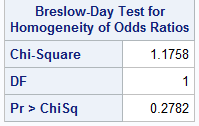
\includegraphics[scale=.6]{bday.png}\\
$\chi^2=1.176$ p-value=$.278>.05$ Fail to reject $H_0$\\
Conclusion: There is not enough evidence to suggest the odds ratios for each sex are not homeogenous. Not enough evidence to suggest a statistically significant difference between the two sexes in the effect of pooled treatment vs placebo on the dichotomized severity of the adverse event none or mild vs. moderate or severe.
\pagebreak
\section*{Problem 3}
\textbf{Under minimal assumptions, conduct a statistical test to determine whether there is a difference in
the proportion of moderate or severe adverse event (vs. none or mild) among the three treatment
groups, controlling for sex. For this problem, you should consider the treatment groups as nominal.
Write a sentence to interpret your findings.}\medbreak

Conducting a Mantel-Haenszel Test\\

$H_0$: There is no difference in the proportions of moderate or severe adverse event (vs. none or mild) among the three treatment
groups, controlling for sex.\\

$\chi^2_{MH}=11.334$ $df=2$ 2 p-value=$.004<.05$ Reject $H_0$\\
Conclude that there is a significant difference in the proportion of moderate or severe adverse event among treatment groups, controlling for sex.\\

\pagebreak
\section*{Problem 4}
\textbf{Under minimal assumptions, conduct a statistical test to determine whether there is a trend in the
proportion of moderate or severe adverse event (vs. none or mild) across the ordered treatment
groups, controlling for sex. Write a sentence to interpret your findings.}\medbreak

Conducting a Mantel-Haenszel Extension Test\\

$H_0$: There is no trend in the proportion of moderate or severe adverse event across the ordered treatment groups, controlling for sex.\\
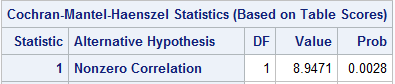
\includegraphics[scale=.6]{qsmh.png}\\
$Q_{CSMH}\sim \chi^2_1=8.947$ p-value=$.003<.05$ Reject $H_0$\\
Conclude there is a statistically significant trend in the proportion of moderate or severe adverse event across the ordered treatment groups, controlling for sex.\\
\pagebreak
\section*{Problem 5}
\textbf{Under minimal assumptions, conduct a statistical test to assess the association of pooled treatment
(high dose + low dose) vs. placebo with the severity of adverse event (all four ordered levels managed
as distinct), controlling for sex. Justify your method. If you determine that $p < 0.05$, discuss whether
pooled treatment is associated with greater severity or lesser severity of the adverse event.}\medbreak

Mantel-Hanszel mean score test\\
Since we cannot assume that the levels of severity of adverse event are equally spaced, we will use modified ridit scores.\\
$H_0$: There is no association of pooled treatment with the ordered severity of adverse event\\
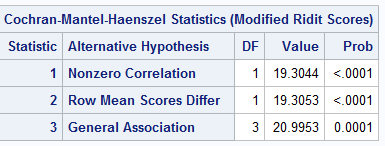
\includegraphics[scale=.6]{modrit.png}\\
$Q_{SMH}\sim \chi^2_1=19.305$ p-value$<.0001$ Reject $H_0$\\
Conclude pooled treatment is associated the ordered severity of adverse event, controlling for sex.\\
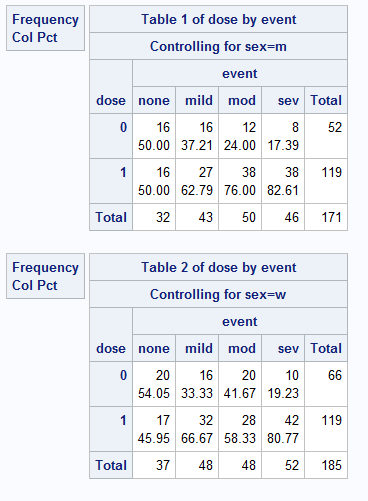
\includegraphics[scale=.6]{tab.png}\\
Looking at the pooled treatment column percentages for each sex, they increase as the level of severity of adverse event increases. Pooled treatment appears to be associated with greater severity of adverse event, while controlling for sex.
\pagebreak
\section*{Problem 6}
\textbf{Under minimal assumptions, conduct a statistical test to determine whether there is a progressive
location shift in the severity of the adverse event (as distinct levels) across high dose, low dose, and
placebo, controlling for sex. In a sentence, interpret your findings.}\medbreak

 Cochran-Mantel-Haenszel test ( Non-Zero Correlation Test)\\
$H_0$: There is no progressive shift in the distribution of the severity severity across
treatment levels controlling for sex.\\
$H_1:$ There is a progressive shift in distribution.\\
$Q_{CSMH}\sim \chi^2_1=17.04$ p-value$<.0001$ Reject $H_0$ \\
Conclude there is a progressive shift in the distribution of the severity severity across
treatment levels controlling for sex.\\
\pagebreak
\section*{Problem 7}
\textbf{Report the Spearman rank correlation coefficients and corresponding 95\% confidence intervals
separately by sex as measures of association for pooled treatment (high dose + low dose) versus
placebo with the severity of adverse event (as distinct levels). Write a sentence indicating whether
men or women exhibit a stronger association, and briefly justify your finding.}\medbreak
\begin{tabular}{|c|c|c|}
	\hline
	Sex & Spearman Rank Correlation & 95\% CI\\
	\hline
	Male&.253 & $(.11,.397)$\\ 
	\hline
	Female&.216 & $(.079,.354)$\\ 
	\hline
\end{tabular}\\
From the table, men in the pooled treatment group have a higher spearman rank correlation than women in the pooled treatment group, this suggests that they have a stronger association than women with severity of adverse event.
\pagebreak
\section*{Problem 8}
\textbf{Report the Spearman rank correlation coefficients and corresponding 95\% confidence intervals
separately by sex as measures of association for ordered treatment groups with severity of the adverse
event (as distinct levels). Write a sentence indicating whether men or women exhibit a stronger
association, and briefly justify your finding.}\medbreak

\begin{tabular}{|c|c|c|}
\hline
Sex & Spearman Rank Correlation & 95\% CI\\
\hline
Male&.222 & $(.07,.373)$\\
\hline
Female&.218 & $(.083,.352)$ \\
\hline
\end{tabular}\\
The results suggest that the associated between increased treatment level and increase severity of event is slightly stronger for men than for women.
\pagebreak
\section*{Problem 9}
\textbf{Separately within each treatment group, test the association between sex and severity of the adverse
event (as ordered distinct levels). Also, assess such association under minimal assumptions, and
controlling for treatment groups. Write a sentence to interpret your results.}\medbreak

Conducting a $\chi^2$ for trend for each treatment group\\
$H_0$: No association between sex and severity of the adverse event\\
Placebo Group:\\
$Q_S\sim \chi^2_1= .135$  p-value=$.713>.05$ Fail to reject $H_0$\\
Low dose group:\\
$Q_S\sim \chi^2_1= .281 $  p-value=$.596>.05$ Fail to reject $H_0$\\
High dose group:\\
$Q_S\sim \chi^2_1= .057$  p-value=$.811>.05$ Fail to reject $H_0$\\
Conclusion: For each treatment group separately we fail to reject the null hypothesis that there is no association between sex and severity of adverse event. This suggests that there is not a statistically significant association between sex and severity of adverse event.
\pagebreak
\section*{Problem 10}
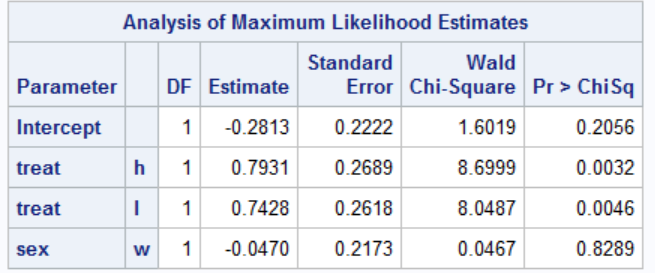
\includegraphics[scale=.6]{logit.png}\\
\textbf{Assumptions:}
Assume data arose from stratified simple random sample so that response is distributed binomially for each
for each treatment x sex combination\\
Each observation is independent from the others\\
The explanatory variables are linearly related to the log odds\\
There is little or no multicollinearity among the explanatory variables\\
\textbf{Explanatory Variables}\\
high indicator of high dose treatment\\
low indicator of low dose treatment\\
(placebo is 0 for both dose indicators)\\
sex indicator of female sex\\
(male is the reference)\\
Response indicator of moderate or severe adverse event\\
$\theta_{hi}$ is the probability that person with hth dose from ith sex has moderate or severe adverse event\\
$logit(\theta_{hi}) = \alpha + \beta_1 I(low) + \beta_2 I(high) + \beta_3 I(female)$\\
$\alpha$ is the intercept, the effect for the reference cell (placebo treatment,female sex)\\
$\beta_1$ is incremental effect for low dose\\
$\beta_2$ is incremental effect for high dose\\
$\beta_3$ is incremental effect for female sex\\
$logit(\theta_{hi}) = -.281 + .743I(low) + .793I(high) +-.047I(female)$\\
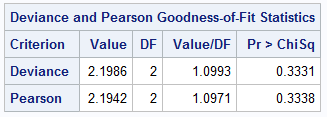
\includegraphics[scale=.6]{gof10.png}\\
$H_0:$ The model is an adequate fit\\
$Q_L=2.199$ p-value=.333 $Q_P=2.194$ p-value=.334\\
both $ Q_L$ and $Q_P$ $\sim \chi^2_{2}$\\
Since both p-values$>.05$ Fail to reject $H_0$, The goodness of fits statistics support the adequacy of the model
\pagebreak
\section*{Problem 11}
\textbf{Using the model from Problem 10, provide estimates and corresponding 95\% confidence intervals
for the odds ratios of high dose vs. placebo and of low dose vs. placebo for (moderate or severe)
adverse event compared to (none or mild).}\medbreak
Odds ratio of high dose vs. placebo for (moderate or severe)
adverse event. $OR=2.21$ 95\% CI: $(1.305,3.744)$\\
Odds ratio of low dose vs. placebo for (moderate or severe)
adverse event. $OR=2.102$ 95\% CI: $(1.258, 3.511)$\\ 
\pagebreak
\section*{Problem 12}
\textbf{Using the model from Problem 10, perform a statistical test of whether the treatment groups differ
with respect to the (moderate or severe) adverse event (i.e., the overall treatment effect). Provide the
test statistic, indicate the number of degrees of freedom, and determine statistical significance
through its p-value. If this overall effect is statistically significant, test each pairwise treatment
comparison at the $\alpha=0.05$ level, and indicate which treatment groups are significantly better than
others. (Note: you do not need to address any adjustment to the type I error for multiple comparisons
for this problem.)}\medbreak
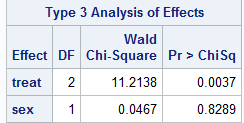
\includegraphics[scale=.6]{type3.png}\\
Running a type 3 wald $\chi^2$ test on the overall treatment effect\\
$H_0:$ The effect of treatment is not significant\\
$\chi^2=11.214$ df=2 p-value=$.004<.05$ Reject $H_0$\\
conclude there the overall effect of treatment on moderate or severe adverse is event is statistically significant.\\
Wald $\chi^2$ test testing pairwise treatment comparisons\\
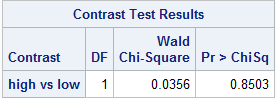
\includegraphics[scale=.6]{highlow.png}\\
High dose vs placebo wald $\chi^2=8.7$ df=1 p-value=$.003<.05$  \\
Low dose vs placebo  wald $\chi^2=8.049$ df=1 p-value=$.005<.05$ \\
High dose vs low dose  wald $\chi^2=.036$ df=1 p-value=$.85>.05$ \\
The results suggest both high dose and low dose are more effective than placebo\\
The difference in treatment effect between high and low dose is not statistically significant.
\pagebreak 
\section*{Problem 13}
\textbf{Using your model from Problem 10, what are the respective model-predicted probabilities for
(moderate or severe) adverse event and for (none or mild) adverse event for men on high dose and
also for women on placebo?}\medbreak
men on high dose $P(\text{moderate of severe})=.602$\\
$P(\text{none or mild})=1-.602=.398$\\
women on placebo $P(\text{moderate of severe})=.419$\\
$P(\text{none or mild})=1-.419=.581$\\
\pagebreak
\section*{Problem 14}
\textbf{Assumptions:}
Data that arise from a stratified simple random sample, at least 5 observations at each outcome at
each level of each main effect, $\beta_k =\beta $ for all k\\
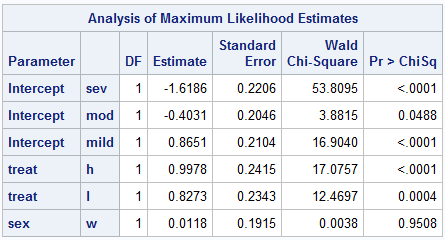
\includegraphics[scale=.6]{propodds.png}\\
$logit(\theta_k)=\alpha_1+\alpha_2+\alpha_3+x_1\beta_1+x_2\beta_2+x_3\beta_3$\\
where $\theta_1$ is P(event=severe)\\
$\theta_2$ is P(event=severe or event =moderate)\\
$\theta_3$ is P(event=severe or event =moderate or event=mild)\\
$\alpha_1$ Intercept for the 1st cumulative logit (log odds of severe event vs moderate, mild or none for males on placebo)\\
$\alpha_2$ Intercept for the 2st cumulative logit (log odds of severe event or moderate vs mild or none for males on placebo)\\
$\alpha_3$ Intercept for the 2st cumulative logit (log odds of severe event or moderate or mild vs none for males on placebo)\\
$x_1=I(\text{treatment=high})$\\
$x_2=I(\text{treatment=low})$\\
$x_3=I(\text{sex=female})$\\
$\beta_1$ Incremental effect for all 3 types of log odds due high dose treatment\\
$\beta_2$ Incremental effect for all 3 types of log odds due low dose treatment\\
$\beta_3$ Incremental effect for all 3 types of log odds due to female sex\\
Score Test for Proportional Odds Assumption\\
$H_0: \beta_k=\beta$ for all k\\
$\chi^2=3.408$ df=6 p-value=$.756>.05$ Fail to reject $H_0$\\
Conclude the overall proportional odds assumption holds\\
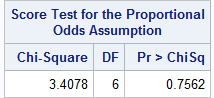
\includegraphics[scale=.6]{stpo.png}
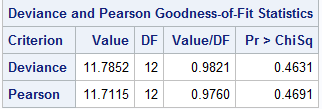
\includegraphics[scale=.6]{gofprop.png}\\
$H_0:$ The model is an adequate fit\\
$Q_L=11.785$ p-value=.463 $Q_P=11.712$ p-value=.469\\
both $ Q_L$ and $Q_P$ $\sim \chi^2_{12}$\\
Since both p-values$>.05$ Fail to reject $H_0$, The goodness of fits statistics support the adequacy of the model
\pagebreak
\section*{Problem 15}
\textbf{Using the model from Problem 14 that assumes proportional odds, provide estimates and
corresponding 95\% confidence intervals for the odds ratios of high dose vs. placebo and of low dose
vs. placebo for (severe or moderate) adverse event compared to (none or mild).}\medbreak
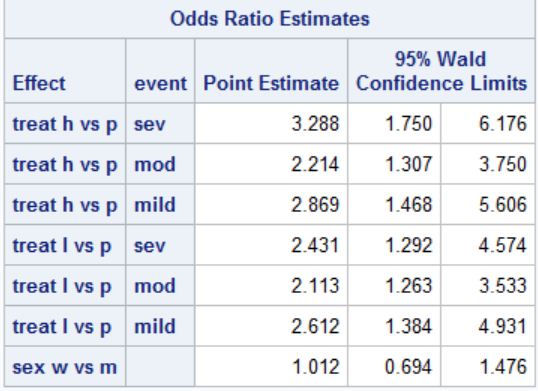
\includegraphics[scale=.6]{partial.png}\\
The odds ratio of high dose vs. placebo for (severe or moderate) adverse event compared to (none or mild) is 2.214 with a 95\% CI $(1.307, 3.750 )$\\
The odds ratio of low dose vs. placebo for (severe or moderate) adverse event compared to (none or mild) is 2.113 with a 95\% CI $(1.263, 3.533)$
\pagebreak
\section*{Problem 16}
\textbf{Using the model from Problem 14 that assumes proportional odds, what are the respective model-
predicted probabilities for none, mild, moderate, and severe adverse event for men on low dose?}\medbreak

\begin{tabular}{|cc|}
	\hline
	Model Predicted probabilities for men on low dose&\\
	\hline
	Severity & Probability\\
	\hline
	None & .696\\
	\hline
	Mild & .845\\
	\hline
	Moderate & .607\\
	\hline
	Severe & .312\\
	\hline
\end{tabular}
\pagebreak
\section*{Problem 17}
\textbf{Assumptions:}\\
Data is from a stratified random sample\\
Treatment is nominal\\
Cell counts are greater than 5\\
observations in the data set are independent\\
model fits the data adequately\\

$logit(\theta_{hij})=\alpha_j+\boldsymbol{x}^{\prime}_{hi}\boldsymbol{\beta}_j$\\
h=1,2,3 for placebo, low, high dose respectively (placebo is the reference)\\
i=1,2 for male and female sex respectively (male is the reference)\\
$\theta_{hij}$ is the odds of event severity with h treatment level and i sex\\
j=1,2,3 where j=1 is the odds of mild vs. none, j=2 is the odds of moderate vs.
none, j=3 is the odds of severe vs. none\\
$x_{1i1}=I(\text{treat=h,j=1})$ \quad $x_{1i2}=I(\text{treat=h,j=2})$ \quad $x_{1i3}=I(\text{treat=h,j=3})$\\
$x_{2i1}=I(\text{treat=l,j=1})$ \quad $x_{2i2}=I(\text{treat=l,j=2})$ \quad $x_{2i3}=I(\text{treat=l,j=3})$\\
$x_{h11}=I(\text{sex=f,j=1})$ \quad $x_{h12}=I(\text{sex=f,j=2})$ \quad $x_{h13}=I(\text{sex=f,j=3})$\\
$\alpha_1=-.121$ intercept for 1st cumulative logit (reference placebo, male sex)\\

$\alpha_2=-.044$ intercept for 2nd cumulative logit (reference placebo, male sex)\\

$\alpha_3=-.724$ intercept for 3rd cumulative logit (reference \ placebo, male sex)\\

$\beta_1=.742$ incremental effect for high dose treatment for $logit_{hi1}$ \\

$\beta_2=.736$ incremental effect for high dose treatment for $logit_{hi2}$\\

$\beta_3=1.725$ incremental effect for high dose treatment for $logit_{hi3}$\\

$\beta_4=.662$ incremental effect for low dose treatment for $logit_{hi1}$ \\

$\beta_5=.854$ incremental effect for low dose treatment for $logit_{hi2}$\\

$\beta_6=1.445$ incremental effect for low dose treatment for $logit_{hi3}$\\

$\beta_7=.005$ incremental effect for female sex for $logit_{hi1}$ \\

$\beta_8=-.135$ incremental effect for female sex for $logit_{hi2}$\\

$\beta_9=.053$ incremental effect for female sex for $logit_{hi3}$\\
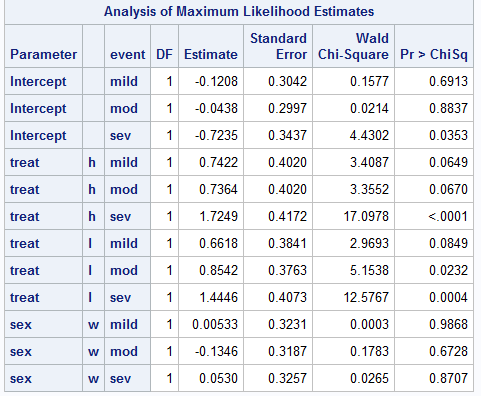
\includegraphics[scale=.6]{glogit.png}\\


\pagebreak
\section*{Problem 18}
\textbf{Using your model from Problem 17, provide estimates and corresponding 95\% confidence intervals
for the odds ratios of high dose vs. placebo and of low dose vs. placebo for each severity level
compared to ‘none’. Compare and contrast these results to those found in Problem 15.}\medbreak
Table of Odds ratio estimates and 95\% CI\\
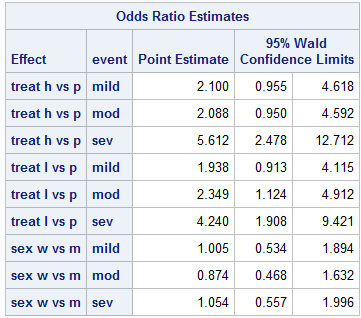
\includegraphics[scale=.6]{org.png}\\
*compared to none event severity\\ 
The odds ratios are similar to the odds ratios in problem 15.
\pagebreak
\part*{Part 2}
\section*{Problem 19}
\textbf{Under minimal assumptions and controlling for baseline falls count in the prior eight weeks
trichotomized as $<5$ falls, 5-10 falls, or $>10$ falls, conduct a statistical test to assess the association
between treatment group and improvement, where improvement is defined as having fewer falls
across the entire eight-week study period than during the preceding eight weeks, and no improvement
is defined as having the same number or more falls. Briefly interpret your results in 1-2 sentences.}\medbreak
Mantel-Haenszel Test\\
$H_0:$ There is no association between treatment group and improvement when controlling for baseline falls. 
 $\chi^2_1=83.234$ p-value$<.0001$ Reject $H_0$\\
 Conclude there is evidence of a statistically significant association between treatment group and improvement when controlling for baseline falls. 
 \pagebreak
\section*{Problem 20}
Fitting a poisson regression model\\
$\log(\mu(x))=x^{\prime}\beta=\beta_0+\beta_1 I(active treatment)+\beta_2 I(tribase1)+\beta_3 I(tribase2)+\beta_4 age$\\
where tribase=1 is $5<baseline falls<10$ tribase=2 is $>10$\\
Table of GOF Statistics\\
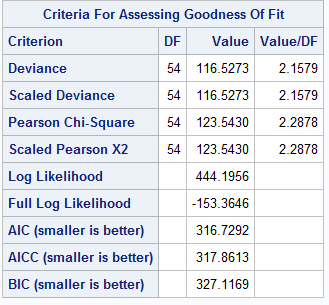
\includegraphics[scale=.6]{gofpois.png}\\
With values of 2.158 for the deviance/df and 2.288 for Pearson/df, there is
evidence of overdispersion.\\
Adjusting for over-dispersion using a scale parameter\\
Table of parameter estimates, standard errors, test statistics and p-values\\
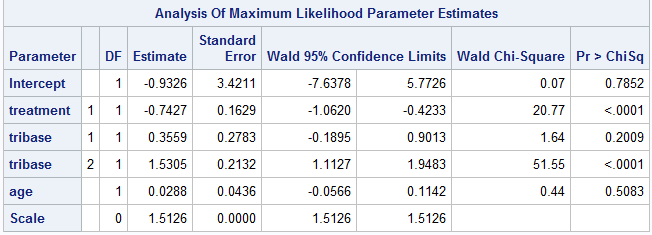
\includegraphics[scale=.6]{pois2.png}\\
Looking at the type 3 analysis we can see that treatment and tribase (trichotomized baseline) are clearly significant where as age appears to not a be statistically significant effect for total count. Adjusting for over-dispersion does not change the parameter estimates, only the standard errors are different.\\
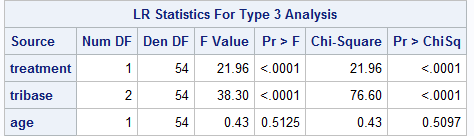
\includegraphics[scale=.6]{typ3pois.png}\\ 
\pagebreak
\section*{Problem 21}
\textbf{Using the model from Problem 20, what is the model-predicted mean falls count during the eight-
	week post-randomization interval for an individual having 5-10 baseline falls in the prior eight
	weeks, who is 80 years old, and was}:
\subsection*{a} \textbf{randomized to receive the experimental treatment}\medbreak
 model-predicted mean falls count:\\
$exp(-.9326+-.7427+.3559+80*.0288)=2.677$

\subsection*{b} \textbf{randomized to receive placebo}\medbreak
 model-predicted mean falls count:\\
$exp(-.9326+.3559+80*.0288)=5.625$
\pagebreak
\section*{Problem 22}
\textbf{ Regardless of your findings regarding over-dispersion in Problem 20, fit a negative binomial model
	to the total falls counts, with the same main effects as specified in Problem 20. For each parameter
	in the model, report the estimate, standard error, test statistic, and p-value. Compare these results to
	those you found in your final model (i.e., adjusted for over-dispersion, if necessary) in Problem 20.}\medbreak
Fitting a negative binomial model to adjust for over-dispersion\\
Table of estimates, standard errors, test statistics, and p-values\\
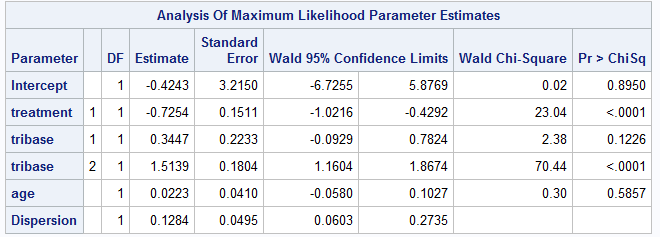
\includegraphics[scale=.6]{nb.png}\\
Comparing the results of the two models the parameter estimates are very similar, the main difference is that the negative binomial model has a larger intercept (-.424 compared to -.933) and the negative binomial model has smaller standard errors, which leads to smaller confidence intervals.
\pagebreak
\part*{Part 3}
\section*{Problem 23}
Fitting a repeated measures Poisson model wiht pairwise treatment interaction terms assuming an exchangeable working correlation structure\\
Model= treatment tribase age time treatment*tribase treatment*age treatment*time\\
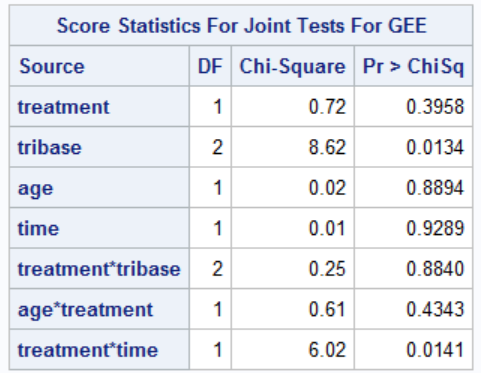
\includegraphics[scale=.6]{score3.png}\\
The Score statistics for Type 3 GEE Analysis Tests show that only the treatment*time interaction is significant.
Refitting the model with the treatment*time interaction\\
Table of parameter estimates\\
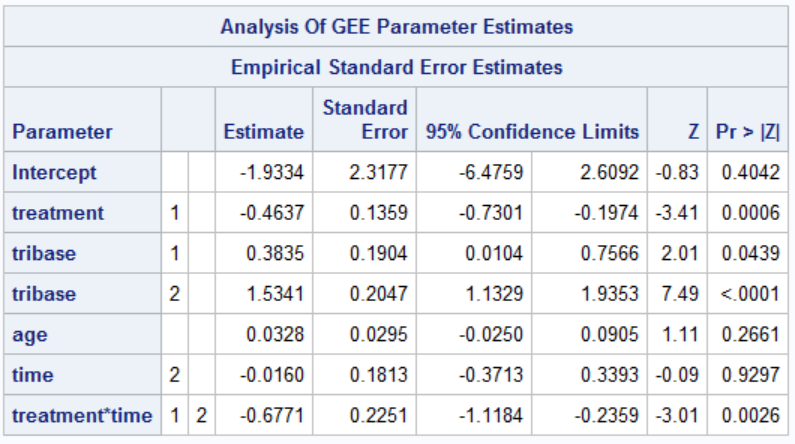
\includegraphics[scale=.6]{gee.png}\\
\pagebreak
\section*{Problem 24}
\textbf{For this problem, you should restate your final recommended model from Problem 23 at the top of
	the page for the grader’s reference. Using this final model, provide the falls rate ratio comparing
	experimental treatment and placebo at each post-randomization period (i.e., for Weeks 1-4 and
	separately for Weeks 5-8), and provide the corresponding 95\% confidence intervals for these
	estimates.}\medbreak
Final Model= treatment tribase age time treatment*time\\
Weeks 1-4 rate ratio=.629 95\% CI:$(.482,.821)$\\ 
Weeks 5-8 rate ratio=.32  95\% CI:$(.195,.525)$\\ 
\pagebreak
\section*{Problem 25}
\textbf{For this problem, you should restate your final recommended model from Problem 23 at the top of
	the page for the grader’s reference. Provide the predicted mean falls count at the Week 5-8 interval
	for an individual having 5-10 baseline eight-week falls, who is 80 years old, and was:}
Final Model= treatment tribase age time treatment*time\\
\subsection*{a} \textbf{randomized to the experimental treatment arm} \medbreak
Predicted mean falls count=$exp(-.016+.0328*80+.3835+-1.9334+(-.4637+-0.6771))=.921$
\subsection*{b} \textbf{randomized to the placebo arm}\medbreak
Predicted mean falls count=$exp(-.016+.0328*80+.3835+-1.9334)=2.881$
\end{flushleft}
\end{document}
